\documentclass{article}
\usepackage[utf8]{inputenc}
\usepackage[brazil]{babel}
\usepackage{indentfirst}
\usepackage{amsmath}
\usepackage{amsthm}
\usepackage{amsfonts}
\usepackage{graphicx}
\usepackage{listings}

\newtheorem*{demo}{Demonstração}
\renewcommand{\d}{\delta}
\newtheorem*{remark}{Observação}
\newtheorem{theo}{Teorema}
\newcommand{\D}{\Delta}
\newcommand{\floor}[1]{\lfloor {#1} \rfloor}
\newcommand{\ceil}[1]{\lceil {#1} \rceil}
\newcommand{\C}{\overline}
\newcommand{\graph}[1][G]{#1 = (V,A)}
\newcommand{\K}[1]{K_{#1}}
\newcommand{\bK}[2]{K_{{#1},{#2}}}
\newcommand{\sg}{\subseteq}

\title{Atividade Extracurricular em Cultura e Extensão\\
       Maratona de programação}
\author{Nathan Benedetto Proença}
\date{\today}

\begin{document}
\maketitle
\section{Andamento geral}

Apresento como resultado as noventa horas prometidas. Pode-se
encontrar informações detalhadas sobre as competições de uma
maneira melhor apresentada e organizada em \texttt{http://nathanpro.github.io/mac0214},
mas irei terminar este documento com a parte ``crua'' da informação
lá contida.

O restante da informação provém do repositório no github em si,
e é em boa parte sobre o que irei discutir e fazer comentários.

Começo com o gráfico que mostra as contribuições para a branch
master do repositório. Ele é um bom termômetro do meu trabalho
durante o semestre, pois em geral o código era adicionado logo
após as competições, e a documentação era feita a posteriori.

\begin{center}
    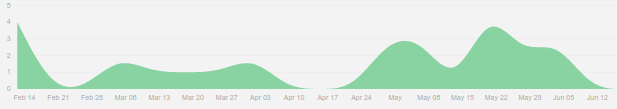
\includegraphics[scale=.55]{andamento}
\end{center}

Este gráfico, por refletir as horas investidas em simulações,
também reflete minha organização pessoal durante o semestre.
Em geral, consigo investir mais tempo em treinos para a maratona
quando as coisas estão em dia, e a curva do gráfico é condizente
com isto.

Na primeira semana do semestre, duas das minhas matérias não
haviam começado. E mesmo após o começo, eu estava com as atividades
relativamente em dia -- por não haverem atividades a serem relizadas.
Conforme foram surgindo as obrigações da graduação, meu tempo de
treino diminuiu, para então se estabilizar.

Há outro ponto onde não houve treino, e este é sempre um momento
crítico de um semestre na graduação: A semana que concentra as
primeiras provas. Entre os dias 4 e 12 de abril tive quatro
avaliações, o que explica a ausência de tempo.

Felizmente, depois destes momentos críticos, consegui colocar
as atividades em dia e encontrar mais momentos na agenda para
treinar.

\section{Resultados numéricos}

A obrigação de organizar e documentar meu treinamento tornou 
possível analisar grande parte da minha produção em código 
durante o semestre.

No repositório há apenas código referente a problemas resolvidos.
Com alguns truques de unix é possível levantar informações
interessantes.

\textbf{Problemas resolvidos total:} 97

\textbf{Linhas de código escritas total:} 3497

\textbf{Competições participadas:} 32

\textbf{Problemas em competições:} 80

\textbf{Linhas de código escritas em competições:} 2585

\textbf{Média de linhas por problema em competição:} 32

\textbf{Problemas foras de competição:} 17

\textbf{Linhas de código escritas em competições:} 912

\textbf{Média de linhas por problema  fora de competição:} 53

\textbf{Problema com menos linhas:} 13

\textbf{Problema com mais linhas:} 86

Destes números, o mais interessante é notar que os problemas fora
de competição tem praticamente o dobro da quantidade de linhas
do que os em competição. Isto reflete o fato de que, ao se treinar
com tempo livre, eu busco resolver problemas mais difíceis, enquanto
numas competição eu foco em primeiro garantir os mais triviais.

\section{Conclusões}

Foi interessante documentar e olhar para meu processo de treinamento.
Sinto que houve um maior foco em competições do que em resolver
problemas com teorias novas, e julgo que isto ocorreu pela forma
a qual decidi abordar esta atividade neste projeto, ou seja,
devido ao foco dado para competições na parte de registro desta
matérias. Normalmente resolvo mais exercícios avulsos do que ocorreu
neste semestre.

É interessante comparar com o semestre passado, no qual fiz desafios
de programação. Para a matérias, resolvi 86 problemas em 4263 linhas
de código, o que dá uma média maior de problemas por código. Isso
reflete o fato de que em desafios não havia uma restrição de tempo
para a entrega das tarefas -- exceto a data da avaliação, claro.

Estas ponderações me levam a concluir que o foco em competições
me fez implementar mais problemas triviais do que é do meu costume.
Isto é negativo, pois estes pouco contribuem para meu crescimento
e aprendizado, e ressaltam a necessidade de estudar e treinar assuntos
em específico.

No entanto, os simulados contribuem e muito para minha estabilidade
emocional em competições. Estou mais produtivo nas competições, um aspecto
positivo do cronograma do semestre. No {\em codeforces}, pela primeira vez
estou numa sequência de 4 contests nos quais apenas subi, estando no momento 
da escrita deste relatório no maior {\em rating} que eu já atingi.
\end{document}
